\Section{preliminaries}{Preliminaries}

The pruning approach that we present in this paper works on Datalog, a general
language that has been used to express static analyses declaratively \cite{Whaley2007,bravenboer}.  Normally,
these analyses are defined using one monolithic Datalog program which
computes an abstract answer to a query.
For us, it will be convenient to consider the Datalog program, which computes the concrete answer to a query,
as distinct from the abstraction, which is applied on the Datalog program to generate an abstract answer.
This separation will allow us to make theoretical
statements comparing the same Datalog program across different
abstractions.

We first define Datalog (\refsec{datalog}), which describes the
computation of a query (think more in the direction of concrete semantics).
Then, we focus on the abstraction (\refsec{abstractions}), which only interacts
with the Datalog program via the input tuples.
Throughout this section, we will use \reffig{graphExample} as a running example.

%%%%%%%%%%%%%%%%%%%%%%%%%%%%%%%%%%%%%%%%%%%%%%%%%%%%%%%%%%%%
\begin{figure}
\begin{center} {\bf Graph Example} \end{center}
{\bf Input relations}:
\[
\begin{array}{ll}
\edge(g,i,j) & \defn{edge from node $i$ to node $j$ in graph $g$} \\
\head(c,i)   & \defn{first element of array $c$ is $i$} \\
\ext(i,c,c') & \defn{$i$ prepended to $c$ yields $c'$: $c' = [i]+c$} \\
\end{array}
\]
{\bf Rules}:
\[
\begin{array}{lcl}
\path(g,[\initNode]). & \\
\path(g,c')           &\dlogUpdate& \path(g,c), \head(c,i), \\
                      &           & \edge(g, i, j), \ext(j, c, c'). \\
\common(g_1,g_2,i)    &\dlogUpdate& \path(g_1,c), \path(g_2,c), \head(c,i). \\
\end{array}
\]
{\bf Query tuple}: $\xo = \common(\Ga,\Gb,3)$. \\
\\
{\bf Constants}: $\sC = \{ \Ga, \Gb, 0, 1, 2, 3, \vec{0}, \vek{01}, \dots \}$.
\\
\\
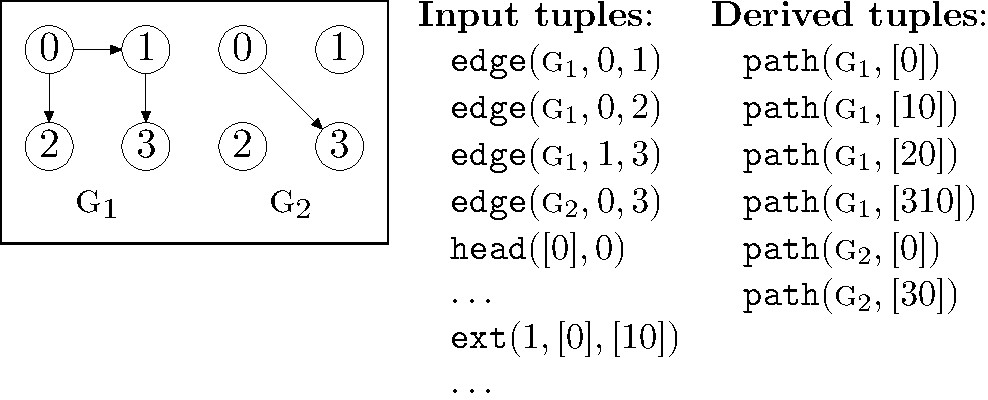
\includegraphics[scale=0.5]{figures/graphExample}
\caption{\label{fig:graphExample}
A simple example illustrating Datalog:
Suppose we have two graphs $\Ga$ and $\Gb$ defined on the same set of nodes $\{0,1,2,3\}$,
and we want to compute the query tuple $\common(\Ga,\Gb,3)$,
asking whether the two graphs have a common path from node $0$ to node $3$.
Given the input tuples encoding the graph,
the Datalog program computes a set of derived tuples from the rules.
In this case, the absence of $\common(\Ga,\Gb,3)$ means the query is false.
}
\end{figure}

%%%%%%%%%%%%%%%%%%%%%%%%%%%%%%
\Subsection{datalog}{Datalog}

A {\em Datalog program} consists of
a set of {\em constants} $\sC$ (e.g., $\initNode,\vec{03} \in \sC$),
a set of {\em variables} $\sV$ (e.g., $i, j \in \sV$), and
a set of {\em relations} $\sR$ (e.g., $\edge \in \sR$).

A {\em term} $t$ consists of a relation $t.r \in \sR$ and a list of arguments $t.\ba$,
where each argument $t.a_i$ is either a variable or a constant,
(that is, $t.a_i \in \sV \cup \sC$) for $i = 1, \dots, |t.\ba|$.
We will write a term in any of the following three equivalent ways:
\begin{align}
t \quad\equiv\quad t.r(t.\ba) \quad\equiv\quad t.r(t.a_1, \dots, t.a_{|t.\ba|}).
\end{align}
For example, $\ext(j,c,c')$ is a term.
We call a term whose arguments are all constants a {\em tuple}
(e.g., $\ext(\initNode, [\,], \vec{\initNode})$).
Note that the tuple includes the relation as well as the arguments.
We let $\xo$ denote a designated {\em query tuple} (e.g., $\common(\Ga,\Gb,3)$),
whose truth value we want to determine.

Let $\sZ$ denote the set of rules,
where each {\em rule} $z \in \sZ$ consists of a target term $z.t$ and a set of source terms $z.\bs$.
We write a rule if $z.t = t$ and $z.\bs = \{ s_1, \dots, s_k \}$ as
\begin{align}
t \dlogUpdate s_1, \dots, s_n.
\end{align}

An {\em assignment} is a function $f : \sV \mapsto \sC$ which maps variables to
constants.  To simplify notation later, we extend an assignment $f$ so that it
can be applied (i) to constants ($f(c) = c$ for $c \in \sC$), and (ii) to terms by
replacing the variables in the term with constants ($f(t) = t.r(f(t.a_1), \dots, f(t.a_{|t.\ba|}))$).

\begin{figure}[ht]
%{\bf Notation:} \\
\[
\begin{array}{ll}
\xo                           & \defn{designated query tuple} \\
\sC                           & \defn{set of concrete values} \\
\bD(X)                        & \defn{derivations using input tuples $X$} \\
\bP(X) \subset X              & \defn{set of relevant input tuples} \\
\alpha : \sC \mapsto \sP(\sC) & \defn{abstraction, maps to equivalence class} \\
A_k \subset \sP(\sC)          & \defn{abstract input tuples after $k$ iterations} \\
\tilde A_k = \bP(A_k)         & \defn{relevant abstract input tuples} \\
\end{array}
\]
\caption{\label{fig:notation} Notation.}
\end{figure}

%%%%%%%%%%%%%%%%%%%%%%%%%%%%%%
%\Subsection{derivations}{Derivations}
\paragraph{Derivations}

A Datalog program takes a set of input tuples and derives new
tuples.  To formalize this computation, we define the notation of a derivation.

A {\em derivation} (of the query $\xo$) with respect to a set of input tuples
$X$ is a sequence $\bx = (x_1, \dots, x_n)$ such that
\begin{enumerate}
\item [(i)] for each $i = 1, \dots, n$, we have $x_i \in X$; or
there exists a set of indices $J$ such that $(J,i)$ satisfies the following conditions:
$j < i$ for each $j \in J$, and
there is a rule $z \in \sZ$ and an assignment $f$
such that $f(z.t) = x_i$ and
$\{ x_j : j \in J \} = \{ f(s) : s \in z.\bs \}$;
\item [(ii)] $x_n = \xo$; and
\item [(iii)] 
for each $j = 1, \dots, n\!-\!1$,
there exists $J$ such that $j \in J$ and an index $i$
such that $(J,i)$ satisfies the conditions in (i).
\end{enumerate}
Define $\bD(X)$ to be the set of all derivations with respect to the input tuples $X$.

% Explain
Condition (i) says that each tuple in a derivation
should either be given as an input tuple ($x_i \in X$)
or be the result of some rule $z \in \sZ$.
Condition (ii) says that $\xo$ was finally produced via some sequence of rule applications.
Condition (iii) says that in the derivation of $x_n$, every tuple is relevant for deriving $\xo$.
%As we will see later, this condition is important because it allow us to
%define the set of irrelevant tuples that can be pruned.

A Datalog program computes $\bD(X)$.
We say that the query $\xo$ is false (proven) if and only if $\bD(X)$ is empty.
Although the query is the ultimate quantity of interest,
the Datalog program can be used to provide more information, which will be useful for pruning.
Specifically, we define $\bP(X)$ to be the subset of the input tuples $X$
which were used in some derivation:
\begin{align}
\label{eqn:Pdef}
\bP(X) \eqdef \{ x \in X : x \in \bx \in \bD(X) \}.
\end{align}
We call $\bP(X)$ the set of {\em relevant input tuples}.  As we will see later,
any tuple not in this set can be safely pruned.
In fact, $\bP(X)$ also tells us whether the query is true or false.
In particular, $\bD(X) = \emptyset$ if and only if $\bP(X) = \emptyset$.
This equivalence suggests that proving and pruning are intimately related;
in some sense, proving the query is just pruning away the query tuple.
In the remainder of the paper, we will make heavy use of $\bP$ as the principal
proving/pruning operation.

%%%%%%%%%%%%%%%%%%%%%%%%%%%%%%
\paragraph{Computation}

We can compute $\bP(X)$ in Datalog by using the Datalog program transformation technique described in 
\cite{liang11minimal}.
This allows us to use off-the-shelf Datalog solvers which have already been optimized
to compute $\bP(X)$.
Specifically, we define a set of new relations $\sR' = \{ r' : r \in \sR \}$.
For a term $t = t.r(t.\ba)$ we let $t' = t.r'(t.\ba)$ be the term that uses the corresponding new relation.
We then add the following new Datalog rules:
\begin{align}
\xo' &\dlogUpdate \xo, \label{eqn:revBase} \\
s'   &\dlogUpdate z.t', z.\bs \quad \text{for each $z \in \sZ$ and $s \in z.\bs$.} \label{eqn:indBase}
\end{align}
The key point is that a tuple $x'$ is derived by the new Datalog program if and only if $x \in \bP(X)$.
These two rules construct $\bP(X)$ recursively:
The base case \refeqn{revBase} states that the query tuple $\xo \in \bP(X)$.
The recursive case \refeqn{indBase} states that if $x \in \bP(X)$ and a rule $z$ (with some assignment $f$)
was used to produce $x$, then for every source term $s \in z.\bs$ of that rule,
we also have $f(s) \in \bP(X)$.

%%%%%%%%%%%%%%%%%%%%%%%%%%%%%%
\Subsection{abstractions}{Abstractions}

Given a Datalog program, we define an {\em abstraction} as a equivalence relation over
the constants $\sC$ (concrete values).  In particular, we represent it as the projection
function which maps each element to its equivalence class (its abstract value):
\begin{definition}
\label{def:abstraction}
An abstraction is a function $\alpha : \sC \to \sP(\sC)$
such that for each set $s \in \range(\alpha)$,
we have $\alpha(c) = s$ for all $c \in s$.
\end{definition}
We use the natural partial order on abstractions,
where $\alpha_1 \preceq \alpha_2$ iff $\alpha_1(c) \supset \alpha_2(c)$ for all $c$,
that is, $\alpha_2$ is finer than $\alpha_1$.

% Example
In the context of our example (\reffig{graphExample}),
we could define an abstraction
that maps a sequence $c$ to the set of sequences that have the same first element as $c$
(e.g., $\alpha([10]) = \{ [1], [10], [11], \dots \}$).
This abstraction is a simplified version of the abstractions we use in our
$k$-limited analyses (see \refsec{abstractionExamples}).

% Extend to sets
We extend $\alpha$ to sets of constants (which we also call abstract values):
\begin{align}
\alpha(s) = \{ \alpha(c) : c \in s \}, \quad s \in \sP(\sC),
\end{align}
which returns a set of abstract values.
This allows us to naturally define compositions of abstractions
by flattening sets of abstract values:
\begin{align}
(\alpha_1 \circ \alpha_2)(c) \eqdef \cup_{s \in \alpha_1(\alpha_2(c))} s.
\end{align}
An important property of equivalence relations is
that if $\alpha_1 \preceq \alpha_2$, then $\alpha_1 \circ \alpha_2 = \alpha_1$
(applying a finer abstraction first has no impact).
Note that in general for arbitrary $\alpha_1,\alpha_2$,
the composition $\alpha_1 \circ \alpha_2$ is not an abstraction;
it is something that we must check when we consider compositions in
\refsec{algorithm}.

% Extend to tuples
We also extend $\alpha$ to concrete tuples $x$ and sets of concrete tuples $X$:
\begin{align}
\alpha(x) &= x.r(\alpha(x.a_1), \dots, \alpha(x.a_{|x.\ba|})), \\
\alpha(X) &= \{ \alpha(x) : x \in X \}.
\end{align}
Here, $\alpha(x)$ is an abstract tuple (one where the arguments are abstract values)
and $\alpha(X)$ is a set of abstract tuples.
For example:
\begin{align}
& \alpha(\ext(1, [0], [10])) = \\
& \quad\quad \ext(1, \{[0], [00], [01], \dots\}, \{[1], [10], [11], \dots\}). \nonumber
\end{align}
Finally, we extend $\alpha$ to abstract tuples $b$ and sets of abstract tuples $B$:
\begin{align}
\alpha(b) &= \{ b.r(s_1, \dots, s_{|b.\ba|}) : \forall i, s_i \in \alpha(b.a_i) \}, \label{eqn:alphab} \\
\alpha(B) &= \cup_{b \in B} \alpha(b). \label{eqn:alphaB}
\end{align}
\refeqn{alphab} applies the abstraction function to each component and takes the cross product over the possible abstract values,
yielding a set of abstract tuples;
\refeqn{alphaB} aggregates these sets of abstract tuples.

Given an abstraction $\alpha$,
we can run an abstract version of the Datalog program to compute an abstract answer to the query tuple.
We do this by applying the abstraction to the concrete input tuples $X$,
to produce a set of abstract input tuples $\alpha(X)$.
We then can feed these tuples into the Datalog program,
which is oblivious to whether the tuples are abstract or concrete;
conceptually, the Datalog program now operates on the constants $\sP(\sC)$ rather than $\sC$.
\reffig{graphDerivation} shows an example of performing this computation on the
graph example from \reffig{graphExample}.

We say the query is proven by $\alpha$ if $\bP(\alpha(X)) = \emptyset$,
and it is proven only if the query is actually false ($\bP(X) = \emptyset$).
This is the standard soundness property, summarized below (see \refapp{proofs} for the proof):
\begin{proposition}[Abstraction is sound]
\label{prop:soundness}
Let $\alpha$ be an abstraction and let $X$ be any set of input tuples.
If $\bP(\alpha(X)) = \emptyset$ (the query is false abstractly),
then $\bP(X) = \emptyset$ (the query is false concretely).
\end{proposition}

\FigStar{figures/graphDerivation}{0.3}{graphDerivation}{
Computation of $\bP(X)$ on the graph example from \reffig{graphExample}
under an abstraction which maps a path onto the set of paths with the same first element
(e.g., $\alpha(\vec{10}) = \{\vec{1}, \vec{10}, \vec{11}, \dots \} \eqdef \vec{1}*$).
Each abstract tuple is derived by a rule whose source terms correspond to the incoming edges.
Relevant input tuples ($\bP(X)$, shown in green) are the ones which are reachable by following the edges backwards;
ones which are not are pruned ($X\backslash\bP(X)$, shown in red).
}
